\documentclass[
% twocolumn,
% hf,
]{ceurart}

%%
%% One can fix some overfulls
\sloppy
\usepackage{xspace}

%%
%% Minted listings support 
%% Need pygment <http://pygments.org/> <http://pypi.python.org/pypi/Pygments>
\usepackage[visiblestringtabs,stylenumbers]{listings}
\usepackage{listings-javascript}
\usepackage{listings-smalltalk}
\lstset{
%  language=JavaScript,
  backgroundcolor=\color{white!95!black},
  extendedchars=true,
  basicstyle=\normalsize\ttfamily,
  numbers=left,
  numberstyle=\scriptsize,
  numbersep=7pt,
  tabsize=4,
  breaklines=false,
  captionpos=b
}
\renewcommand{\ttdefault}{pcr}
%% auto break lines
%\lstset{breaklines=true}


\def\secref{$\S$\ref}
\def\Secref{$\S$\ref}
\def\figref{figure~\ref}
\def\Figref{Figure~\ref}
\def\tabref{table~\ref}
\def\Tabref{Table~\ref}

\newcommand{\code}[1]{\textsf{#1}}
\newcommand{\js}{Javascript\xspace}
\newcommand{\jvm}{JVM\xspace}
\newcommand{\thejvm}{the JVM\xspace}
\newcommand{\Thejvm}{The JVM\xspace}
\newcommand{\java}{Java\xspace}
\newcommand{\ph}{Pharo\xspace}
\newcommand{\pjs}{PharoJS\xspace}
\newcommand{\pjvm}{PharoJVM\xspace}
\newcommand{\st}{Smalltalk\xspace}
\newcommand{\py}{Python\xspace}
\newcommand{\cpp}{C++\xspace}

%%
%% end of the preamble, start of the body of the document source.
%\global\let\Citeauthor=\relax 
%\global\let\bibfont=\relax 
%\global\let\bibhang=\relax 
%\global\let\citename=\relax 
%\usepackage{biblatex}
% \addbibresource{biblio.bib}
%\addbibresource{dls.bib}
%\addbibresource{popl.bib}
%\addbibresource{lncs.bib}
%\addbibresource{wikipedia.bib}
%\addbibresource{misc.bib}
%\addbibresource{ieee.bib}
%\addbibresource{oopsla.bib}
%\addbibresource{books.bib}
%\addbibresource{sigplan.bib}

{\makeatletter
  \gdef\@ceurLogoLine{}
}
\begin{document}

%%
%% Rights management information.
%% CC-BY is default license.
\copyrightyear{2022}
\copyrightclause{Copyright for this paper by its authors.
  Use permitted under Creative Commons License Attribution 4.0
  International (CC BY 4.0).}

%%
%% This command is for the conference information
\conference{International Workshop on Smalltalk Technnology 2022 (IWST22)}

%%
%% The "title" command
\title{Design Principles for a High-Performance Smalltalk}

%\tnotemark[1]
%\tnotetext[1]{You can use this document as the template for preparing your
%  publication. We recommend using the latest version of the ceurart style.}

%%
%% The "author" command and its associated commands are used to define
%% the authors and their affiliations.
\author{Dave Mason}[
orcid=0000-0002-2688-7856,
email=dmason@ryerson.ca,
]
%\affiliation{%
%  \institution{Toronto Metropolitan University}
%  \city{Toronto}
%  \country{Canada}
%  }

\address{Toronto Metropolitan University, Toronto, Canada}

%%
%% The abstract is a short summary of the work to be presented in the
%% article.
\begin{abstract}
  In its 40+ years of existence, there have been many implementations of Smalltalk and related languages, with many different design goals.
  Most have emphasized its best-in-breed development environment and its rich class library.

  A few have focussed more on performance and/or generating stand-alone code.
  The system described in this paper falls in the latter camp.
  This paper describes the work-in-progress and the design principles that are focussed in the short term on generating high-performance stanalone executables from an applicationi developed within a Pharo environment.
  Future goals include being able to support a live IDE based on the OpenSmalltalk clients: Pharo/Squeak/Cuis.
\end{abstract}

%%
%% Keywords. The author(s) should pick words that accurately describe
%% the work being presented. Separate the keywords with commas.
\begin{keywords}
interpreter
compiler
runtime environment
\end{keywords}

%%
%% This command processes the author and affiliation and title
%% information and builds the first part of the formatted document.
\maketitle

\section{Introduction}
Smalltalk was created and iterated through the 1970s\cite{10.1145/3386335}, culminating in Smalltalk-80\cite{Smalltalk-80,10.5555/226}.
Smalltalk-80 was the version that was commercialized along corporate pathways that culminated in products by Cincom\cite{Cincom-smalltalk} and Instantiations\cite{Instantiations-smalltalk} (many other commercial versions exist, notably GemStoneS\cite{Gemtalk-smalltalk}).
A version of Smalltalk-80 was also used as the basis for ANSI~Standard INCITS 319-1998\cite{ANSI-Smalltalk}.

Because the commercial versions were not very accessible, many ``FOSS'' versions have also been produced, mostly based on specification in the ``Blue Book''\cite{Smalltalk-80}.
The most widely available versions are Pharo\cite{Pharo-Smalltalk}, Squeak\cite{Squeak-Smalltalk}, and Cuis\cite{Cuis-Smalltalk}, all of which run on the Opensmalltalk-VM (see \secref{openst}).

There are many parts of what makes up ``Smalltalk'':
\begin{enumerate}
\item The language is one of the simplest of programming languages, with the syntax famously ``completely visible on a postcard''.
  There are only 2 kinds of statements: expressions, and returns (with assignment being a kind of expression).
  All the control structures are semantically simply the sending of messages.
  A straight-forward compiler to byte-codes is quite simple to build.\footnote{...although many tricks are applied to get good performance.}
\item The image.
  Most Smalltalk systems are live environments where browsers, debuggers, inspectors, and compilers are all simply ways at looking at live objects running in the system.
\item A rich library of classes, including dozens of kinds of collections, which have extremely coherent APIs because of the ``duck-typing'' aspect of the dynamic type system.
\item The virtual machine, which interprets the byte-codes or compiles them to native code (typically in a JIT model).
\end{enumerate}

In the 2017 Stackoverflow Developers Survey\cite{stackoverflow-survey-2017}, Smalltalk was the second most loved language.
A very common experience is that people who program in Smalltalk want to program everything in Smalltalk.
There are a couple of ways this can be achieved:
\begin{enumerate}
\item Add features to the Smalltalk environments to support the particular use case, and program/run the application within Smalltalk.
  One way of doing this is to use ``Foreign Function Interfaces'' (FFIs) to access system libraries.
  Another way is building systems like the extremely powerful Seaside Web Framework\cite{Seaside-server} in Smalltalk itself.
\item But sometimes there are constraints that require running code in particular environments.
  Examples include:
  \begin{itemize}
  \item PharoJS - ``Develop in Smalltalk, Run on Javascript'' where one develops code in the rich Pharo IDE, and then generates Javascript to run either in a web browser or a NodeJS server (see \secref{pharojs}).
  \item GNU-Smalltalk - allows writing scripts in Smalltalk, but they load and execute as command-line scripting applications (see \secref{gnu-st}).
  \item Strongtalk - generates very high-performance native executable code, to address performance requirements (see \secref{strongtalk}).
  \end{itemize}
  Here the programmer wants to program as much as possible in Smalltalk and then export the code to another environment where it will run.
\end{enumerate}

\section{Design Principles}
These are the design principles that we believe are relevant to a Smalltalk VM in 2022.
\paragraph{Large memories}
Memory has become extremely inexpensive, and desktops and even smartphones have gigabyes of main memory.
Caches are critical, although remain difficult to optimize for, however having a thread's heap and stack fit comfortably within any per-core L1 cache is an obvious goal.
Large datasets are a significant parts of modern computing, so memory management must be tuned so these can be accessed and released without causing memory bloat.
\paragraph{64-bit and IEEE-768}
64 bit processors and IEEE-768 floating point are becoming ubiquitous.
This makes parametric polymorphism (i.e. having all parameters be the same size) an obvious thing to do.
Floating point is becoming more important, so we want to avoid allocating floating values on the heap.
Fortunately, NaN-boxing as described in \secref{immediate-values} works well.
\paragraph{Multi-core and threading}
Processors are not likely to get appreciably faster any time soon.
The only way to continue to get speedup for applications is to exploit multi-core architectures.
This means both efficient support for computational threads on separate cores without any global interpreter locks.
It is also critical to have a parallel garbage collector that can run with minimal interaction among threads.
\paragraph{Fast execution}
For a dynamically-typed, late-binding language like Smalltalk to be taken seriously for many applications, it must have good performance.
Part of this is having fast method dispatch, to minimize the cost of that late binding.
The other part is to have largish methods to allow optimizers to perform well.

\section{Zag Smalltalk}

The rest of this paper describes the Zag Smalltalk system.
The current goal is to generate code from a Pharo-written application that can load into a runtime, be compiled as a stand-alone application, and run.
The runtime and the generated code are in the Zig language\cite{zig-lang}.

Zag is intended to run on modern, multi-core, 64 bit architectures.

There are many interesting details about the interpreter and run-time, but the rest of this paper will focus on important principles that we believe make this system unique and will lead to excellent performance.

\subsection{Immediate Values}\label{immediate-values}

Immediate values are instances of classes that have constrained or no instance variables or indexable fields - some of which may have singleton values.
Examples are SmallInteger, Double, Boolean, and Character.
Since we are assuming all values are 64-bit values, it is natural to consider if there are ways to encode all values in 64 bits and to minimize the objects that have to be allocated in memory.
Everything that can be coded as an immediate value is something that doesn't have to be garbage collected.

It turns out that the IEEE floating point format - which is ubiquitous - has a lot of holes called Not-A-Number or NaN values.
\Figref{IEEE-fp} shows the IEEE-754\cite{ieee-754} 64-bit binary floating point number format.
All the values where the exponent is 0x7FF are considered NaN (except for one positive and one negative infinity value), and these can be used for any purpose other than as valid floating point.
\begin{figure}[htbp]\label{IEEE-fp}
  \caption{Bit pattern for IEEE-754 64-bit floating-point numbers}
  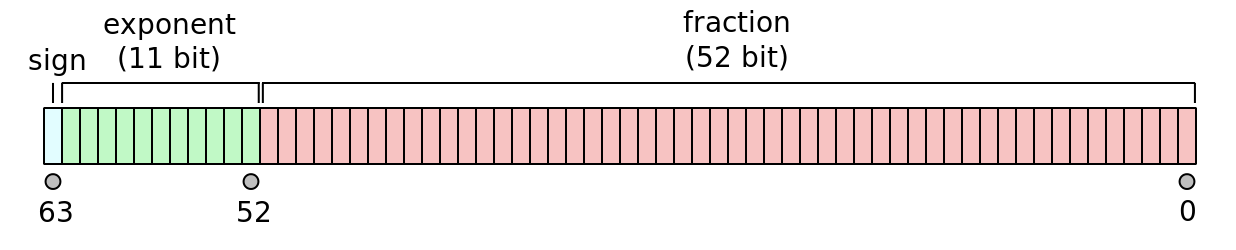
\includegraphics[width=15cm]{IEEE.png}
\end{figure}
This is a technique called NaN-boxing\cite{nan-boxing-duperas,nan-boxing-nystrom}.

There are two of these NaN ranges - positive and negative - however using just the negative range gives us a lot of flexibility, and improves the speed with which we can recognize the class of an immediate value.
\Tabref{immediates} shows the allocated ranges.
All the non-float values are coded within the negative NaN range - i.e. where the top 12 bits are 0xFFF.
The next 4 bits being 6 denote a reference to a heap-allocated object header, explained in \secref{heap-objects}.  
The next 4 bits being 7 represent general classes - these could be used for any class that had 32-bit unique hash values.
The next 4 bits being 8-15 denote SmallInteger values.

Discovering the class of an immediate value is easy and efficient, considering the value as a unsigned 64-bit (u64) value.
\begin{enumerate}
\item if it is greater or equal to than \verb|SmallInteger minVal|, it's a SmallInteger (class 2);
\item if it is less than or equal to \verb|-inf| value, it's a Double (class 3);
\item if it is less than the high heap object address, it's a heap object and we need to look at the header to determine the class;
\item extract bits 32-47 and that is the class number
\end{enumerate}
These are done in this order because SmallIntegers are the most common values.

\begin{table}[htbp]\label{immediates}
  \caption{Mapping of IEEE 64-bit floats to Smalltalk Immediate Values}
  \begin{tabular}{l|l|l|l|l}
 S+E       & F    & F    & F    & Type            \\
\hline
 0000      & 0000 & 0000 & 0000 & double  +0      \\
 0000-7FEF & xxxx & xxxx & xxxx & double (positive)         \\
 7FF0      & 0000 & 0000 & 0000 & +inf            \\
 7FF0-F    & xxxx & xxxx & xxxx & NaN (unused)    \\
 8000      & 0000 & 0000 & 0000 & double     -0   \\
 8000-FFEF & xxxx & xxxx & xxxx & double (negative)         \\
 FFF0      & 0000 & 0000 & 0000 & -inf            \\
 FFF0-5      & xxxx & xxxx & xxxx & NaN (currently unused)\\
 FFF6      & xxxx & xxxx & xxxx & heap object \\
 FFF7      & 0001 & xxxx & xxxx & reserved (tag = Object) \\
 FFF7      & 0002 & xxxx & xxxx & reserved (tag = SmallInteger) \\
 FFF7      & 0003 & xxxx & xxxx & reserved (tag = Double) \\
 FFF7      & 0004 & 0001 & 0000 & False \\
 FFF7      & 0005 & 0010 & 0001 & True \\
 FFF7      & 0006 & 0100 & 0002 & UndefinedObject \\
 FFF7      & 0007 & aaxx & xxxx & Symbol \\
 FFF7      & 0008 & 00xx & xxxx & Character \\
 FFF8-F      & xxxx & xxxx & xxxx & SmallInteger \\
 FFF8      & 0000 & 0000 & 0000 & SmallInteger minVal\\
 FFFC      & 0000 & 0000 & 0000 & SmallInteger  0\\
 FFFF      & FFFF & FFFF & FFFF & SmallInteger maxVal\\

  \end{tabular}
\end{table}

\paragraph{Singleton Values}
The encodings of \verb|nil|, \verb|false|, and \verb|true| are the sole representatives of their respective classes.
Similar encoding could be used for any other classes with singleton values, or indeed any with only a 32 bit payload.
\paragraph{Symbols}
Symbols are encoded very efficiently so that method dispatch can be as fast as possible.
The low 24 bits of the immediate value encode the symbol number, which can be used to access the string representation of the symbol.
The next 8 bits encode the arity of the symbol so that operations like \verb|perform:| can execute without having to access the string representation.
Together, the low 32 bits of the symbol constiture its hash value and method dispatch uses that directly - see \secref{unified-dispatch}.
\paragraph{Character}
All possible Unicode characters are encoded in the hash value of Character immediate objects.
\paragraph{Heap Objects}
The low 48 bits encode the memory address of a heap object header.
To convert an immediate heap value into the address, a simple sign extension of the 48 bits gives a full address for today's commodity hardware.
Another  3 bits are available if/when a larger range is required because every heap object is on at least 8-byte boundaries, so the low 3 bits are 0.
\paragraph{SmallInteger}
This gives 51-bit SmallIntegers (less than the 61-bit SmallIntegers in the OpenSmalltalkVM, but still a very large range).
Converting between tagged SmallIntegers and untagged integers is a simple matter of adding or subtracting the SmallInteger 0 value.

Having SmallIntegers organized this way provides many efficiencies:
\begin{itemize}
\item all of the comparison operations between two SmallIntegers work naturally (i.e. without having to convert to normal integers);
\item adding/subtracting a normal (in-range) integer to/from a SmallInteger works naturally (detect under/overflow if the result is less than \verb|SmallInteger minVal|)
\item adding/subtracting a small normal integer constant (like +/- 1) to/from a SmallInteger that we know is moderate in size doesn't need to be under/overflow checked because the range of SmallInteger is so large;
\item for immediate values \verb|basicIdentityHash| will just be the values or'ed with \verb|SmallInteger 0|, which will turn any value into a positive SmallInteger;
\item \verb|or|, \verb|xor|, etc. with positive normal integers will work naturally;
\item \verb|or|, \verb|and| with tagged positive integers will work naturally.
\end{itemize}

\subsection{Multi-core Support}\label{multi-core}
As is well known, per-processor speed is no longer advancing significantly, so all performance advances in the future are expected to be from using multi-core architectures to their limits.
To the best of our knowledge, most Smalltalk systems continue to only support cooperative process context switching.

Since we are looking for very high performance, we are structuring our system from the outset with support for multiple operating-system threads.
This means that user-written code will have to use synchronization primitives to control access to shared data.
However there is very little additional syncronization required by the runtime infrastructure, beyond memory allocation described in \secref{heap-allocation}.
Only the interning of a new symbol, or manipulation of the dispatch tables described in \secref{unified-dispatch} requires any other kind of global lock.

There are 3 kinds of operating system threads used by the system: mutator, collector, and I/O.
\paragraph{Mutator threads}
These are the main execution threads.
Each mutator thread has its own stack and local heap.
The heap is organized as a small nursery arena where most allocations take place (currently about 3k objects).
The stack is in the top of this area and grows down toward the nursery heap.

Each thread has a lock, and the thread will block on this lock when interacting with other threads.
The thread checks at opportune times during execution to see if another thread wants to interact.
A compute-bound job would typically allocate as many threads as it could use, up to 1 less than the number of CPU cores available.
\paragraph{Global Collector thread}
The global collector periodically performs a mark-sweep collection on the global arena.
It interacts with the mutator threads to determine the roots for collection, as described in \secref{heap-allocation}.
\paragraph{Input/Output threads}
Any blocking operations with the operating system will done by I/O threads, because they do not have to interact with the global collector.
If a mutator thread needs a blocking operation, it requests the appropriate I/O thread to do the operation, leaving a reference to itself, and then blocks on its lock.
When the I/O thread has completed the work, it indicates this to the mutator thread and wakes it up.

\subsection{Heap Allocation}\label{heap-allocation} 
As mentioned in \secref{multi-core}, this system is designed to support multiple threads, with minimal interference.
Since these arenas are unique to the thread, there is no interference or interaction with other threads, so allocation is simply checking for overflow, then storing the values and advancing the heap pointer.
If at any point allocation for the heap or stack would cause those pointers to cross, the live data is copied to the current of two somewhat larger thread-local intermediate (teen) arenas (about 9k objects), the stack area will be adjusted by any forwarded objects, and some of the contexts on the stack could be moved to the teen heap if the stack is getting too big.
Live data is copied back and forth between these teen arenas until they become too full or an object has been copied 8 times, at which point older data is copied to the global arena.

The global arena is a non-moving mark-and-sweep arena, and a thread is dedicated to periodically collecting this arena.
There are no pointers from the global arena to any of the per-thread arenas.
The global arena uses a similar structure to Mist\cite{mist-smalltalk}, which is to say it maintains a set of linked lists of objects of particular sizes.
Instead of the binary-sized blocks that Mist uses, Zag uses fibonacci-sized blocks.

For example, if we need a block for an object of size 15 we would look in the list for the next fibonacci number (21), and if not found, we'd see if the next-sized list had any, and so-on up.
If we find a larger block, we split it into the 2 smaller blocks and put them in the appropriate linked lists.
If we don't find a larger block, we request a new block of memory from the operating system, allocate it into the appropriate lists and then search again.
So in our example we would take a block of size 21, allocate the first 15 to the object, the next 5 into the 5-list, and 1 word unusable.

For objects with arrays larger than about 2k words (16KiB), the array portion will be allocated its own block of pages, and the object will have a remote reference to the block.
The advantage of this is that when the object goes away, we can release its block of pages back to the operating system and reduce memory footprint.
If the large data were to be allocated in the object itself, odds are it would never be possible to release the memory because it would get intermingled with small objects.

\paragraph{Mutator/Collector thread interactions}
At the start of the mark phase, the global arena collector first scans known global structures for roots: the class table, the dispatch table, the symbol table, and the thread table.

Then it iterates to collect roots from the mutator threads:
\begin{enumerate}
\item set a flag in each mutator thread to say it wants roots;
\item when the mutator notices, it will do a collection and then find the first 100 global objects referenced by the stack/heap; then if there are more global references, it will block;
\item the collector looks for mutators that have provided their global objects, and marks all of them (oring 1 into the age field), then wakes up the thread if it has blocked
\item when all the mutators have provided their root global references, the mark phase is complete.
\end{enumerate}

While the mark phase is proceeding, allocations can still be made, they are simply allocated as marked.

During the sweep phase, allocations can be made if there are appropriately-sized block available, but a mutator thread would block rather than request a new block from the operating system.
The sweep phase then goes through memory accumulating blocks of unmarked memory.
If any of the components of that unused memory include references to indirect blocks, those indirect blocks are put into a list for release.
Each accumulated block of memory discovered is then parcelled out to the appropriate fibonacci-size lists.
Each marked allocation has the mark cleared.

Once the sweep phase is complete, allocations are fully enabled and any blocked mutator threads are awakened.
All the indirect blocks that were discovered to be unused are returned to the operating system.
Then the collector pauses for a short period and then starts the cycle over again.

\subsection{Heap Objects}\label{heap-objects}

We are inspired by some of the basic ideas from the SPUR\cite{spur-memory} encoding for objects on the heap, used by the OpenSmalltalk VM (see \secref{openst}).

First we have the object format tag. The bits code the following:
\begin{itemize}
\item bit 0-4: encode indexable fields
\begin{itemize}
	\item 0: no indexable fields
	\item 1: 64-bit indexable no pointers - native words (DoubleWordArray,DoubleArray,) or non-pointer Objects (Array)
	\item 2-3: 32-bit indexable - low bit encodes unused half-words at end (WordArray, IntegerArray, FloatArray, WideString)
	\item 4-7: 16-bit indexable - low 2 bits encode unused quarter-words at end (DoubleByteArray)
	\item 8-15: byte indexable - low 3 bits encode unused bytes at end (ByteArray, String)
	\item 17: 64-bit indexable with some pointers - (Array)
\end{itemize}
\item bit 5-6: encode instance variables
\begin{itemize}
	\item  0: no instance variable
	\item 32: instance variables - no pointers
	\item 64: instance variables - pointers
	\item 96: weak (implying instance variables) - pointers - even if there aren't, because weak values are rare, and they only exist to hold pointers
\end{itemize}
\item bit 7: = 1 says the value is immutable
\end{itemize}

Therefore, only the following values currently have meaning:
\begin{itemize}
\item 32,64: non-indexable objects with inst vars (Association et al) 
\item 1-17: indexable objects with no inst vars
\item 33-49,65-81: indexable objects with inst vars (MethodContext AdditionalMethodState et al)
\item 96: weak non-indexable objects with inst vars  (Ephemeron)
\item 97-113: weak indexable objects with inst vars (WeakArray et al)
\end{itemize}

Note that we differentiate for objects that contain no pointers, either in the instance variables or the indexable values.
This means that if the format anded with 80 = 0, there are no pointers, and garbage collect can skip over the fields without having to scan for pointers (and if it {\em does} scan and finds no pointers, it changes the format to say there are no pointers).
Heap objects are initially created as their pointer-free version.
If a pointer is being stored in an object:
\begin{itemize}
\item if the object is immutable, throw an exception;
\item if storing into the indexable part of a format 2-15 object, throw an exception;
\item if the object has a pointer-free format, update it to pointer-containing;
\item if the object is on the global heap, then the pointed-to object must be promoted to the global arena, recursively.
\end{itemize}

If there are both instVars and indexable fields, the length field is the number of instVars which are followed by a word containing the size of the indexable portion, which follows.
Weak objects are rare enough that we don't bother to handle cases with no instance variables separately.

If there aren't both  instVars and indexable fields, the size is determined by the length field. The only difference between instVars and indexables is whether `at:`, `size`, etc. should work or give an error.

If the array length is >= 4094 (whether in the length field or the additional size word), the values are indirect, and the object will simply contain a size, the address of the indirect block, and an entry in the linked list of indirect objects.
This can only occur in the global arena, so any such large objects are allocated immediately in the global arena.

\Tabref{header-word} describes the header-word for an object.

If the length field is 4095, then this is a forwarding pointer, and the low 48 bits are the address of the real object.
This can occur for several reasons:
\begin{itemize}
\item during mutator arena copying collection, when an object is copied, a forwarding pointer is left behind so other references to the same object can be updated properly;
\item if a value is promoted from a mutator arena to the global arena, a forwarding pointer is left behind;
\item if a \verb_become:_ exchanges two objects, the forward pointer will point to an exchange object.
\end{itemize}

\begin{table}\label{header-word}
  \caption{Object header layout}
  \begin{tabular}{c|l|l}
 Bits &  What         &  Characteristics\\
\hline
    12   &  length       &  number of long-words beyond the header\\
    4 & age & 0 - nursery, 1-7 teen, 8+ global \\
 8    &   format & see above\\
 24   &  identityHash &\\
 16   &  classIndex   &  LSB\\
  \end{tabular}
\end{table}

\subsubsection{Some Particular Heap Objects}
\paragraph{Contexts}
Contexts are allocated on the stack, but may be promoted to the teen arena, for example if \verb_thisContext_ is referenced, or if the stack becomes too large.
\paragraph{Strings}
Strings are stored as UTF-8 sequences or as ASCII sequences.
If a String contains any non-ASCII sequence, it must be scanned to determine its size, or to index it, and is immutable.


\subsection{Unified Dispatch}\label{unified-dispatch}

One of the things that is expected to most significantly improve performance is the unified - or single-level - dispatch.
Every class will have the full set of methods that it has been asked to respond to.
When a message is sent to an object the hash value for the selector symbol will be used to hash into the dispatch table.

This is analogous to how dispatch works in a statically-typed language like Java.
In Java, a method call is associated with a direct integer index into the dispatch or v-table.
For a variety of reasons, this is not possible for a language like Smalltalk.
However, it can be approximated with a hash from the selector to a corresponding entry in the v-table.
The v-table is chosen to be large enough to create a ``perfect'' hash - one with no conflicts (though there may be gaps).
If it's not found, it will be searched for in the class and super-classes - if found it will be compiled and added to the dispatch table.
This means that once stabilized, all message dispatches will require a single hash to access the method.

\subsection{High-Performance Inlining}

When a method is being generated, messages sent to self, as well as methods with few versions, can be inlined.
This will have a similar, but much more significant and principled, effect to the current inlining of special methods like \verb|iftrue:ifFalse:|.

This is a fundamental requirement for high-performance compilation.
Contrast this with the traditional Smalltalk code with only a few message sends per method - this is great for developers, but death to optimizers.

For example a method with a \verb_collect:thenSelect:_ where we know the class of the receiver would inline the method replacing the block parameters with the actual block code.
Then the \verb_to:do:_ would be inlined, which contains a \verb_whileTrue:_ which would be inlined as a loop (because it is a recursive definition).
Then the parameters to the blocks would be inlined.
All the references to \verb_self_ including \verb_class_, \verb_size_ and \verb_at:_ would be inlined.
With some dead-code elimination and recognition that the numbers can all be converted to native values and that the index passed to \verb_at:_ is guaranteed to be in the valid range, this becomes a loop very close to the most efficient possible loop.

\subsection{Code Generation}
We are pusuing two approaches to code generation.
\paragraph{Threaded execution}
To support the full reflective model of execution, but with better performance than available from a traditional interpreter, in the full interpretive model we are using threaded execution.
Threaded execution codes a method as a sequence of function addresses, each of which calls on to the next.
This is quite convenient to do in Zig\cite{zig-lang} as it has explicit support for tail calls.
\begin{figure}[htbp]\label{pushConst}
  \caption{Zig code for {\tt pushConst} primitive}
\begin{verbatim}
    pub fn pushConst(pc: [*]const Code, tos: [*]Object, heap: [*]Object,
                                  thread: *Thread, caller: Context) Object {
        checkSpace(pc,tos,heap,thread,caller,1);
        const newTos = tos-1;
        newTos[0]=pc[0].object;
        return @call(tailCall,pc[1].prim,.{pc+2,newTos,heap,thread,caller});
    }
\end{verbatim}
\end{figure}
\Figref{pushConst} shows an example of a threaded function.
Each function in a \verb_Code_ block has the same parameters: a pointer to the next ``instruction'', stack and heap pointers, a reference to the current Thread, and the caller's context.
This function copies the next object from the code to the top of stack, and then passes control to the next function (``prim''), passing the modified function pointer and stack, as well as the rest of the parameters.
\begin{figure}[htbp]\label{trivial-code}
  \caption{A trivial sequence of threaded code}
\begin{verbatim}
        p.pushConst,3,
        p.pushConst,4,            
        p.p110,
        return_tos,
\end{verbatim}
\end{figure}
\Figref{trivial-code} shows what a sequence of threaded code might look like.
This pushes two objects (3 and 4) on the stack and then does primitive 110 (\verb_==_) and we expect \verb_false_ as the result.

This model can be easily single-stepped and is amenable to other tools.
\paragraph{Exported Zig code}
The other way we are currently exporting code is as Zig programs that can be compiled and linked against the runtime and produce stand-alone executable programs.
This is currently only useful for benchmarking and exploring what a JIT could be expected to produce.

\section{Related Work}
\subsection{Opensmalltalk-VM\cite{10.1145/3281287.3281295,opensmalltalk-github}}\label{openst}
OpenSmalltalk-VM is a virtual machine (VM) for languages in the Smalltalk family (e.g. Squeak, Pharo) which is itself written in a subset of Smalltalk that can easily be translated to C.
Development is done in Smalltalk.
The production VM is derived by translating the core VM code to C.

This is the VM that underlies the Pharo, Squeak, Cuis, and Newspeak systems.
It is a high quality VM implementation including a JIT compiler, but doesn't attain the performance of a similar model such as the V8 Javascript interpreter or NodeJS.
It also has significant dependencies on a single hardware execution thread.

\subsection{GNU-Smalltalk\cite{gnu-st}}\label{gnu-st}
GNU Smalltalk inspired the overall structure of the heap for Zag.
Historically it has run in a strictly stanalone/scripting mode, but an IDE has become available.

\subsection{StrongTalk\cite{10.1145/165854.165893}}\label{strongtalk}
Strongtalk was a very high-performance Smalltalk system that included partial-typing.
This type information was part of what made it so fast.
Unfortunately, the project was abandoned.

\subsection{PharoJS\cite{pharojs}}\label{pharojs}
PharoJS inspired some of the ideas here, such as generating a stand-alone module (in the PharoJS case, to run on a web browser), as well as the mechanism for bringing in all the necessary classes and methods.

\subsection{Mist\cite{mist-smalltalk}}\label{mist}
Mist inspired important aspects of the global arena of the heap. Unfortunately, it appears to have been abandoned.

\subsection{GildaVM\cite{Polito2019GildaVMAN}}\label{gilda}
GildaVm explores some interesting approaches to minimize the effect of a Global Interpreter Lock as a way to bring multiple threading to OpenSmalltalk (see \secref{openst}).
This is to offset the known problems of the GIL that have been well documented in the Python world.

\section{Status and Future Work}
The current goal is to generate code from a Pharo-written application that can load into a runtime, be compiled as a stand-alone application, and run.
We can currently run trivial, hand-compiled, programs.

Once the code generator is working, there are a variety of experiments to run, including determining how significant the unified dispatch and inlining are in affecting performance.
We are very interested in benchmarking against Strongtalk.

In the longer term we intend to do JIT code generation and be able to add new methods to a dispatch table dynamically.
Then we will be working on generating a fully-functional system using one of the open-source Smalltalk IDEs.

Another avenue is integrating a type-inference system so that the inliner can generate many more opportunities for optimization.

%\printbibliography
%\bibliography{dls,popl,lncs,wikipedia,misc,ieee,oopsla,books,sigplan,iwst}
\bibliography{all}
\end{document}
%--- Local Variables: 
%--- coding: utf-8
%--- mode: latex
%--- fill-column: 1000
%--- TeX-master: "main"
%--- TeX-PDF-mode: t
%--- End:
